\begin{figure}[t]
\centering

%------------------ Example A: image_030 ------------------
% Left: original (spans the height of two rows)
\begin{minipage}[c]{0.16\linewidth}
  \centering
  
\includegraphics[width=\linewidth]{figures/mnist_split_ic_saliency/image_030_true_3_pred_3/original.png}\\[-2pt]
  {\scriptsize Original}
\end{minipage}\hspace{0.01\linewidth}%
% Right: two rows of five logits
\begin{minipage}[c]{0.81\linewidth}
  \centering
  % Row 1: logits 0..4
  \begin{minipage}[b]{0.19\linewidth}\centering
    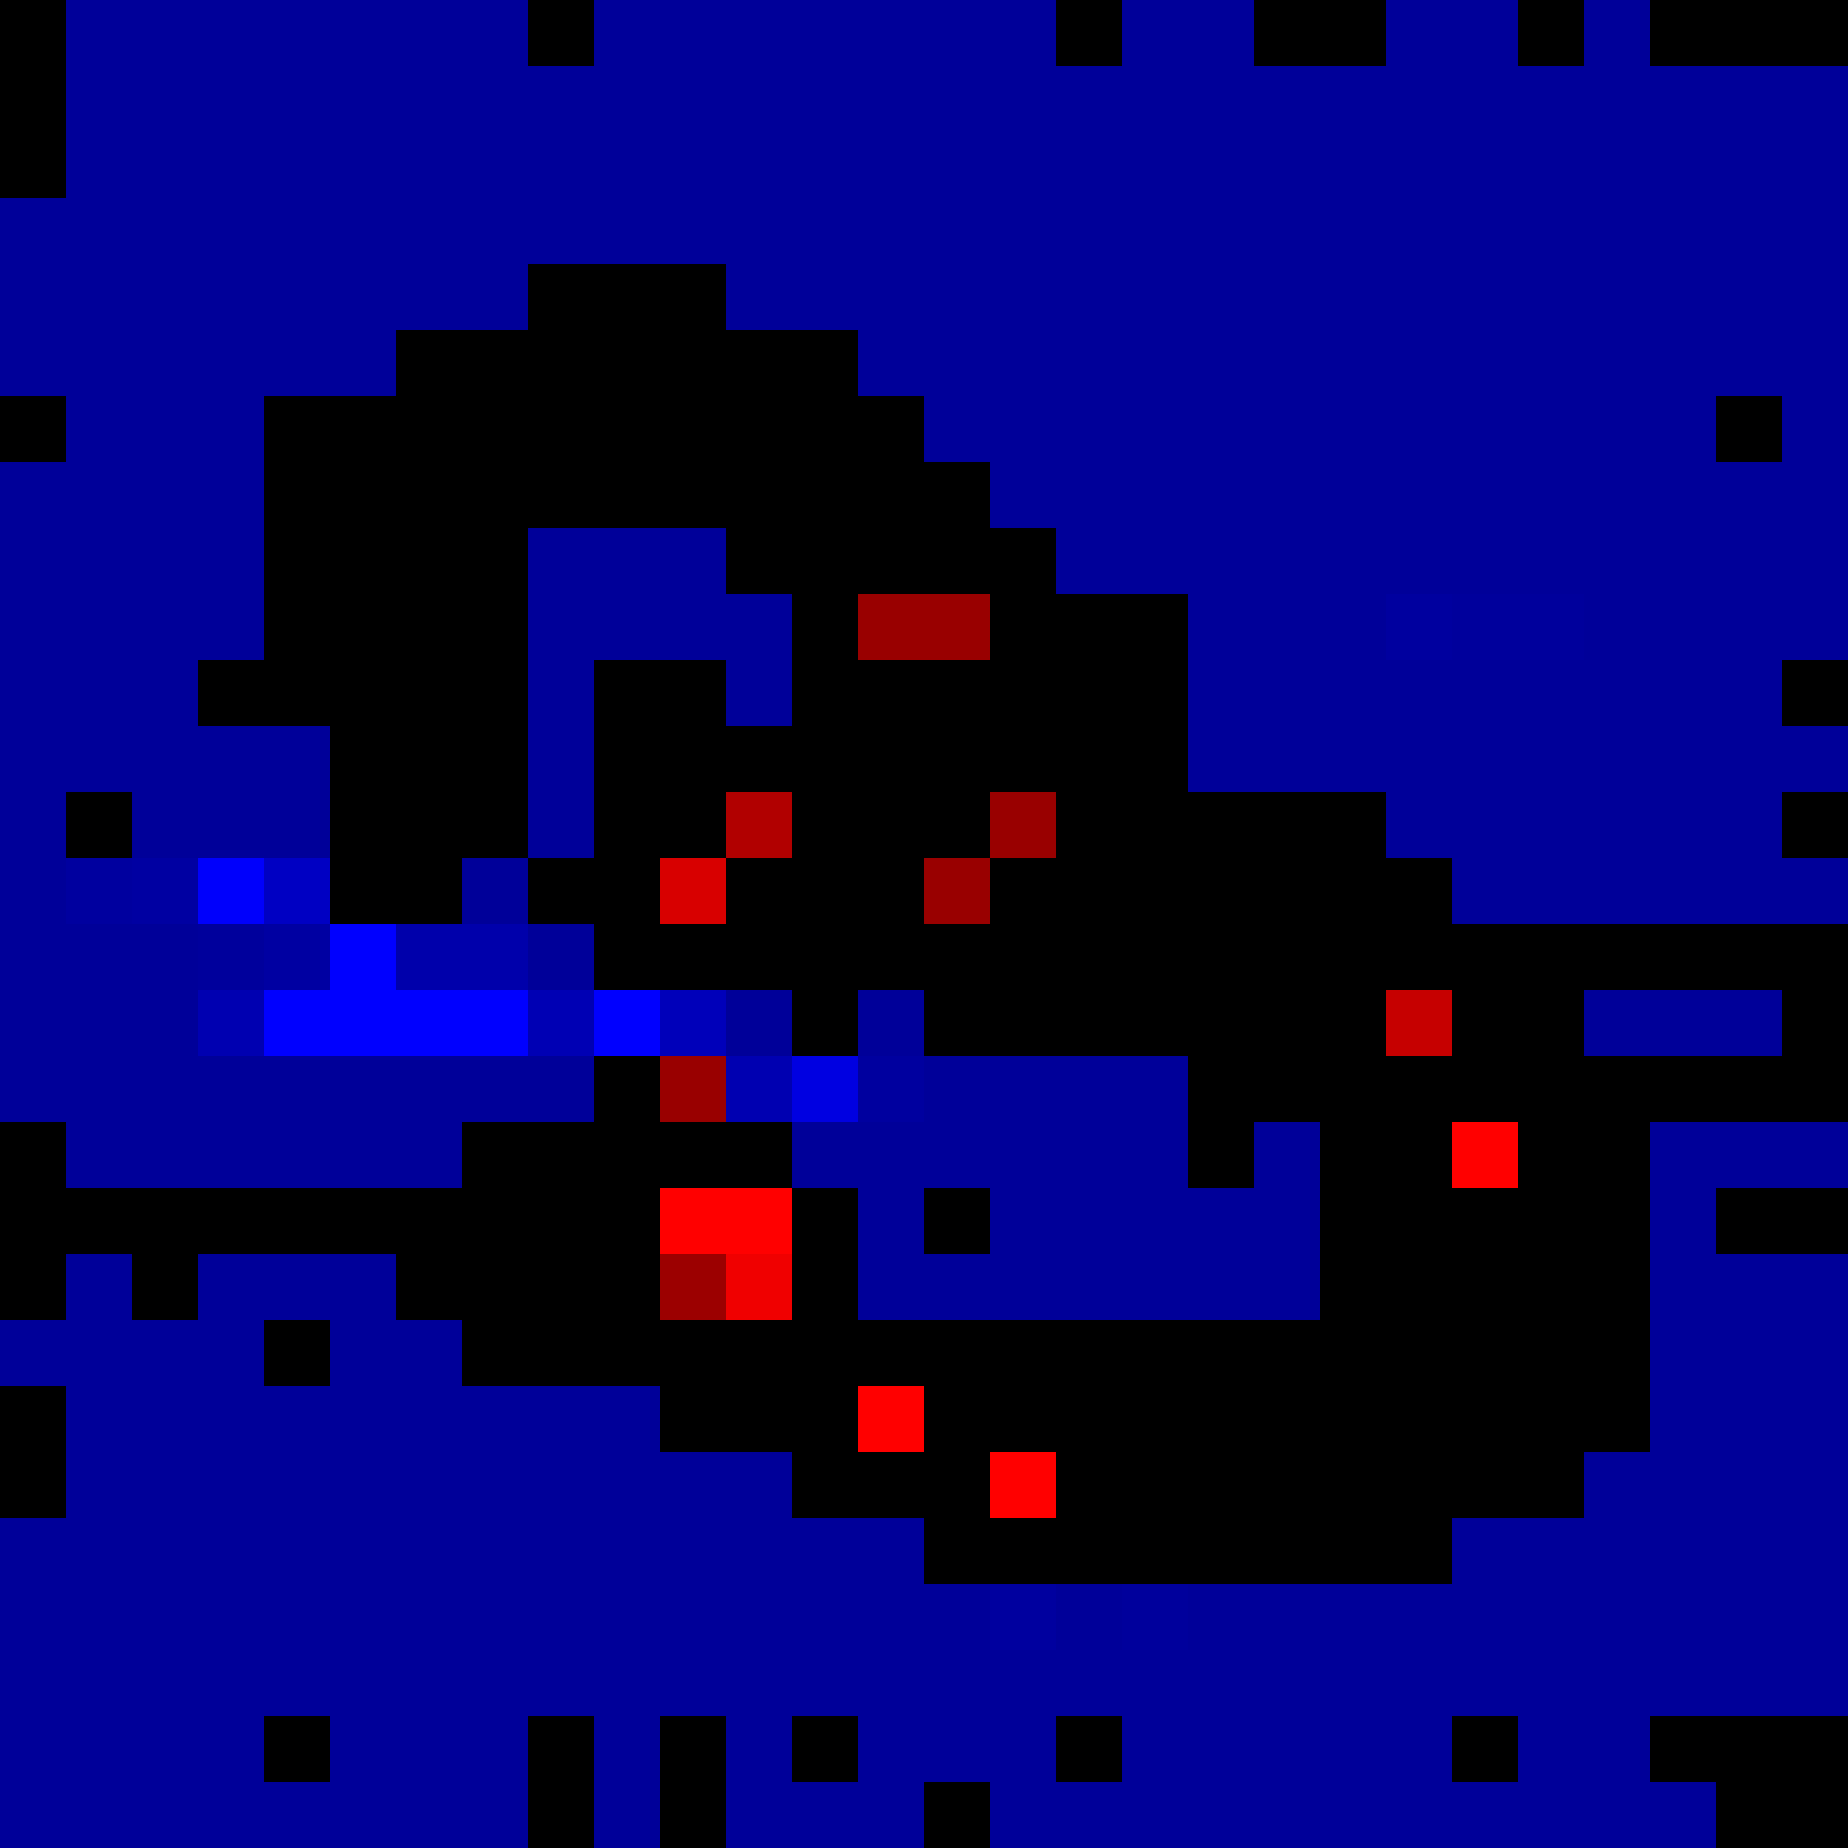
\includegraphics[width=\linewidth]{figures/mnist_split_ic_saliency/image_030_true_3_pred_3/final_saliency_threshold_wrt_0_bright.png}\\[-2pt]{\scriptsize Logit 0}
  \end{minipage}%
  \begin{minipage}[b]{0.19\linewidth}\centering
    
\includegraphics[width=\linewidth]{figures/mnist_split_ic_saliency/image_030_true_3_pred_3/final_saliency_threshold_wrt_1_bright.png}\\[-2pt]{\scriptsize Logit 1}
  \end{minipage}%
  \begin{minipage}[b]{0.19\linewidth}\centering
    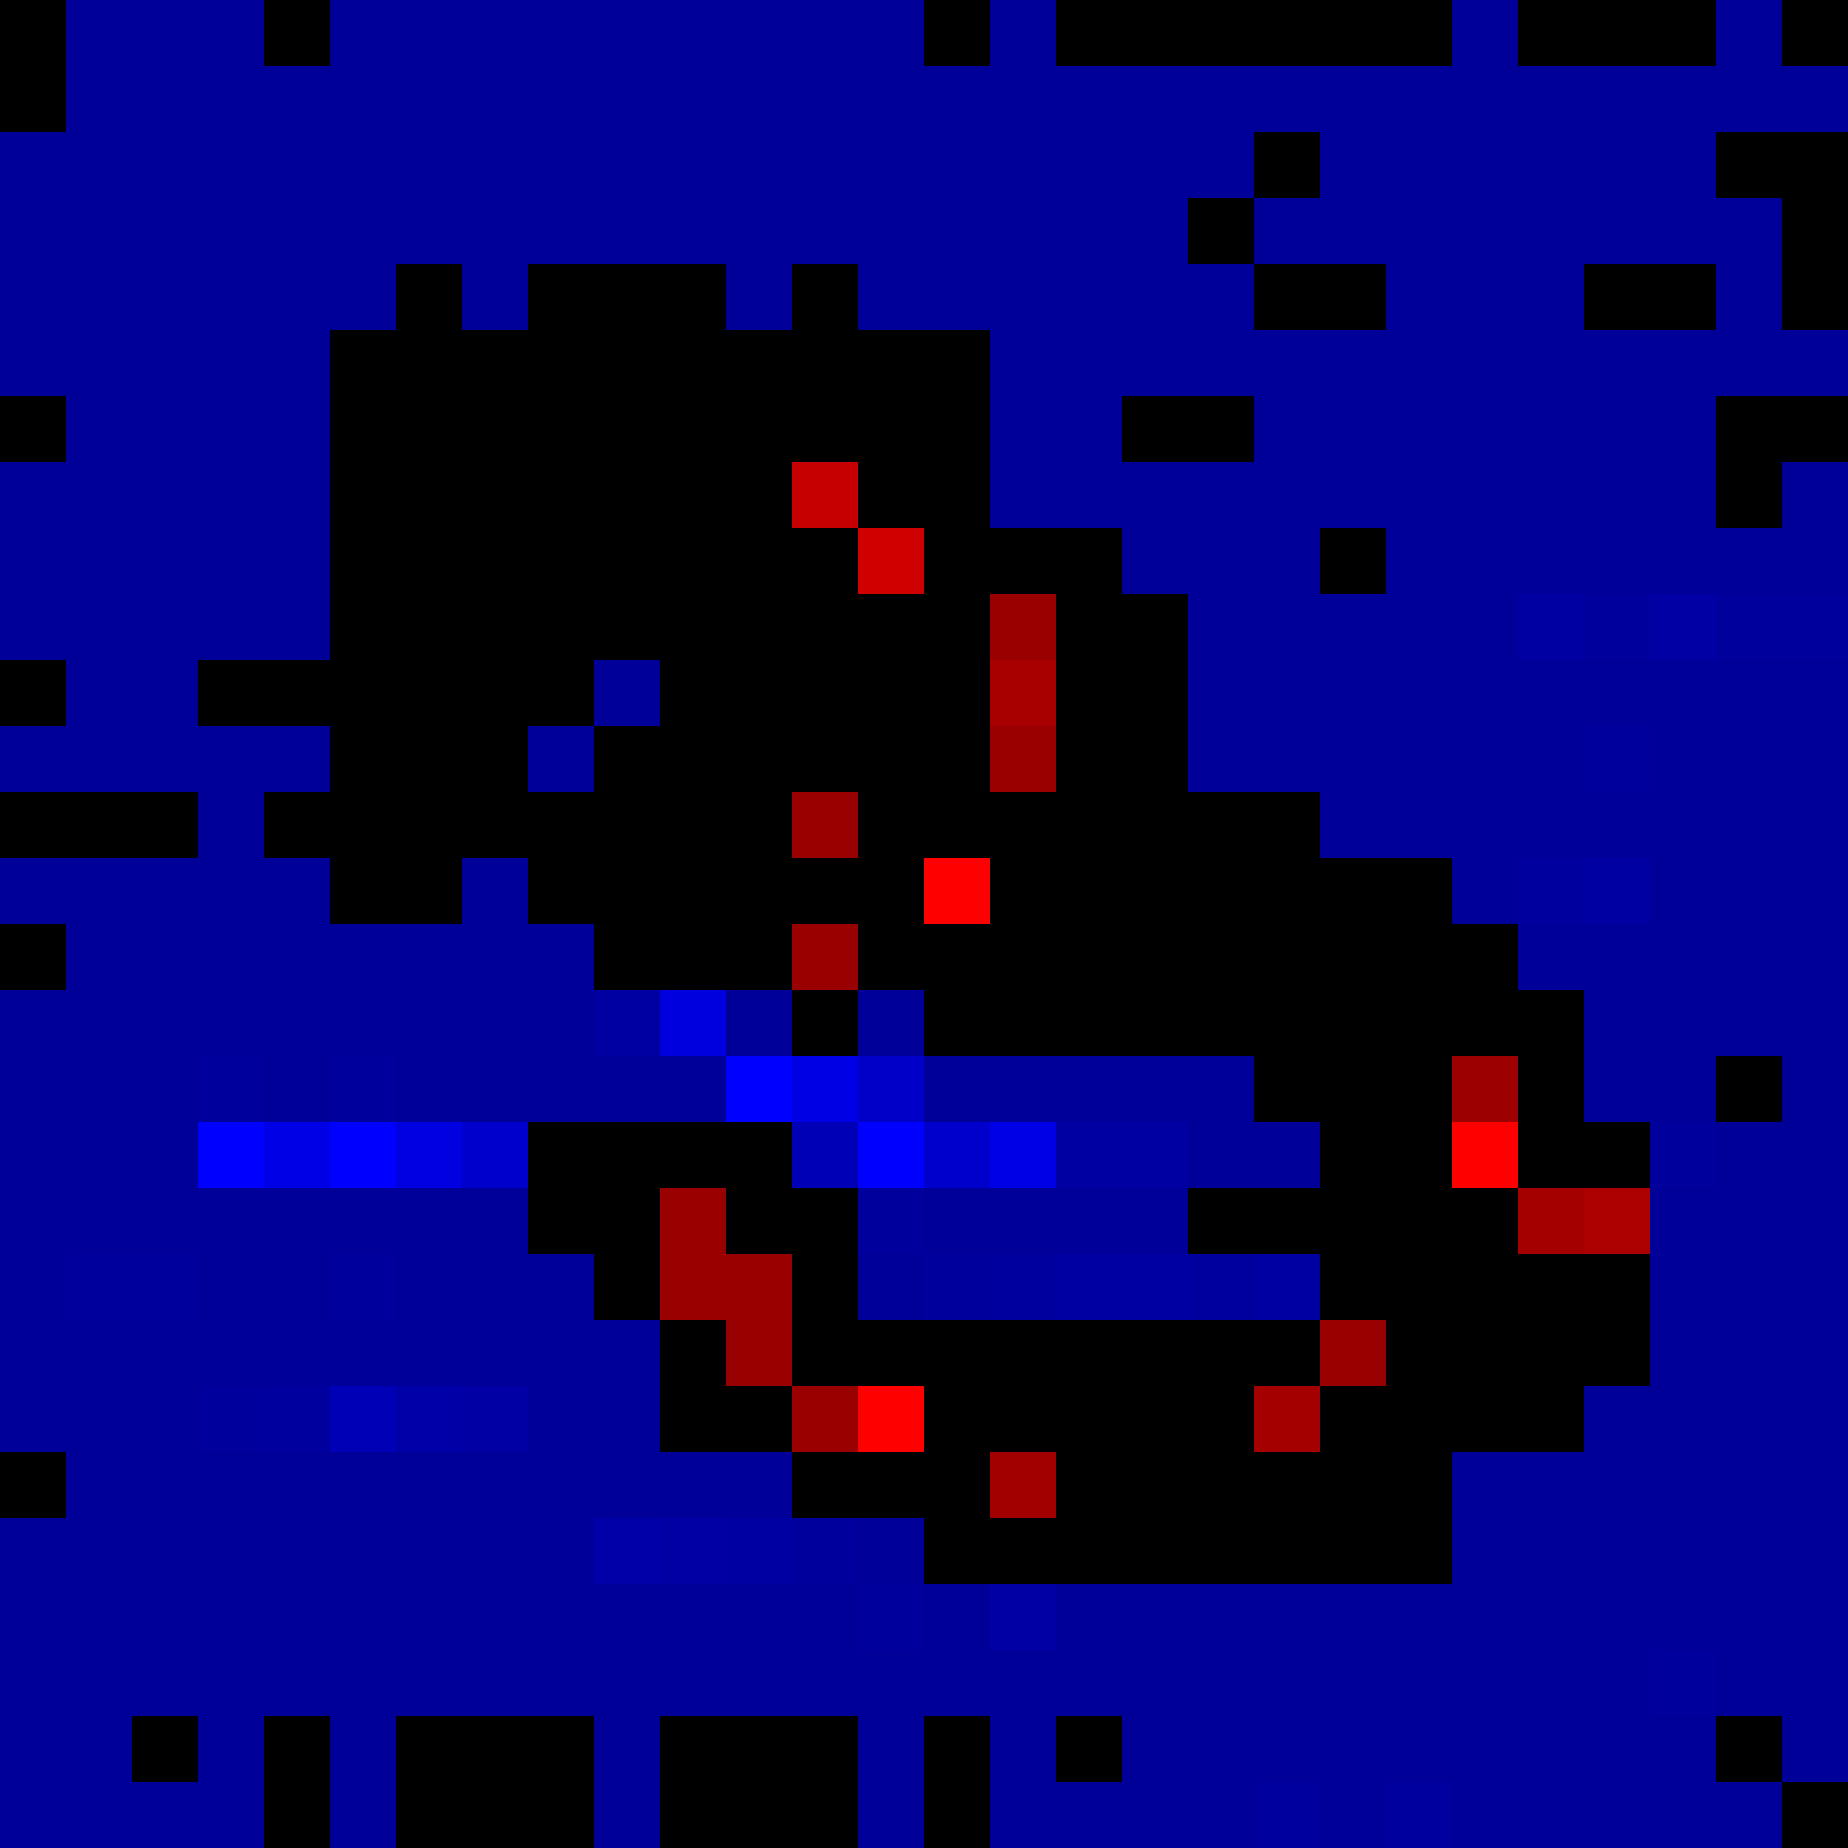
\includegraphics[width=\linewidth]{figures/mnist_split_ic_saliency/image_030_true_3_pred_3/final_saliency_threshold_wrt_2_bright.png}\\[-2pt]{\scriptsize Logit 2}
  \end{minipage}%
  \begin{minipage}[b]{0.19\linewidth}\centering
    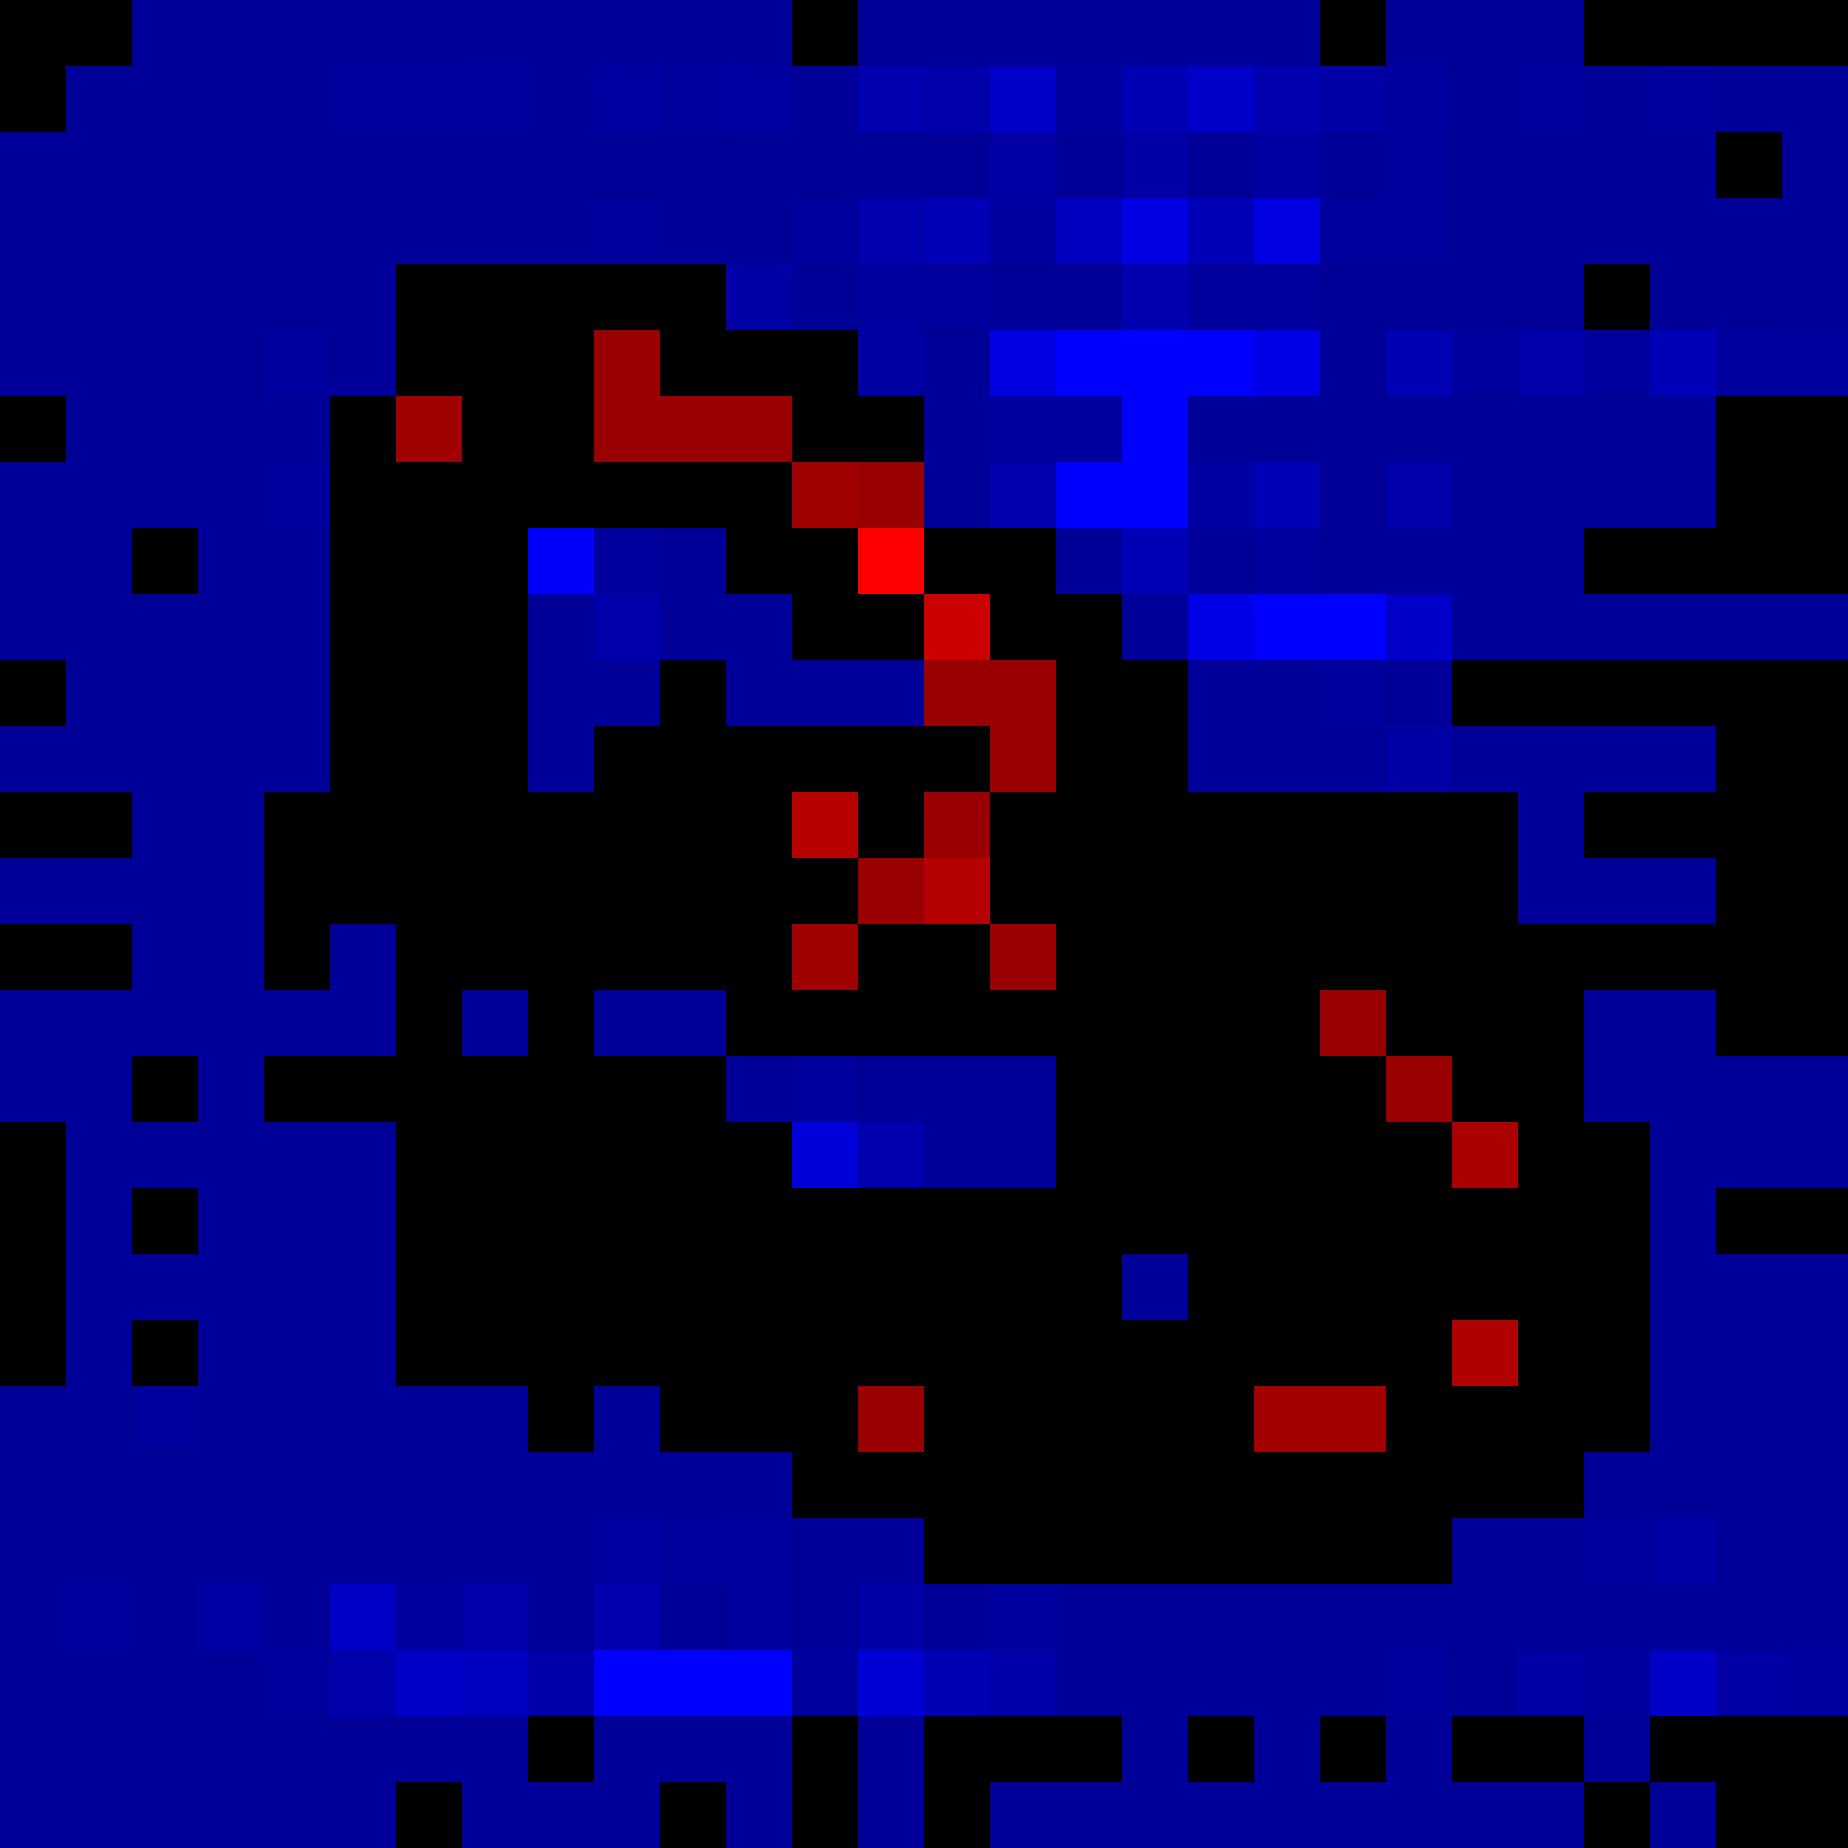
\includegraphics[width=\linewidth]{figures/mnist_split_ic_saliency/image_030_true_3_pred_3/final_saliency_threshold_wrt_3_bright.png}\\[-2pt]{\scriptsize Logit 3}
  \end{minipage}%
  \begin{minipage}[b]{0.19\linewidth}\centering
    
\includegraphics[width=\linewidth]{figures/mnist_split_ic_saliency/image_030_true_3_pred_3/final_saliency_threshold_wrt_4_bright.png}\\[-2pt]{\scriptsize Logit 4}
  \end{minipage}

  \vspace{0.12cm}

  % Row 2: logits 5..9
  \begin{minipage}[b]{0.19\linewidth}\centering
    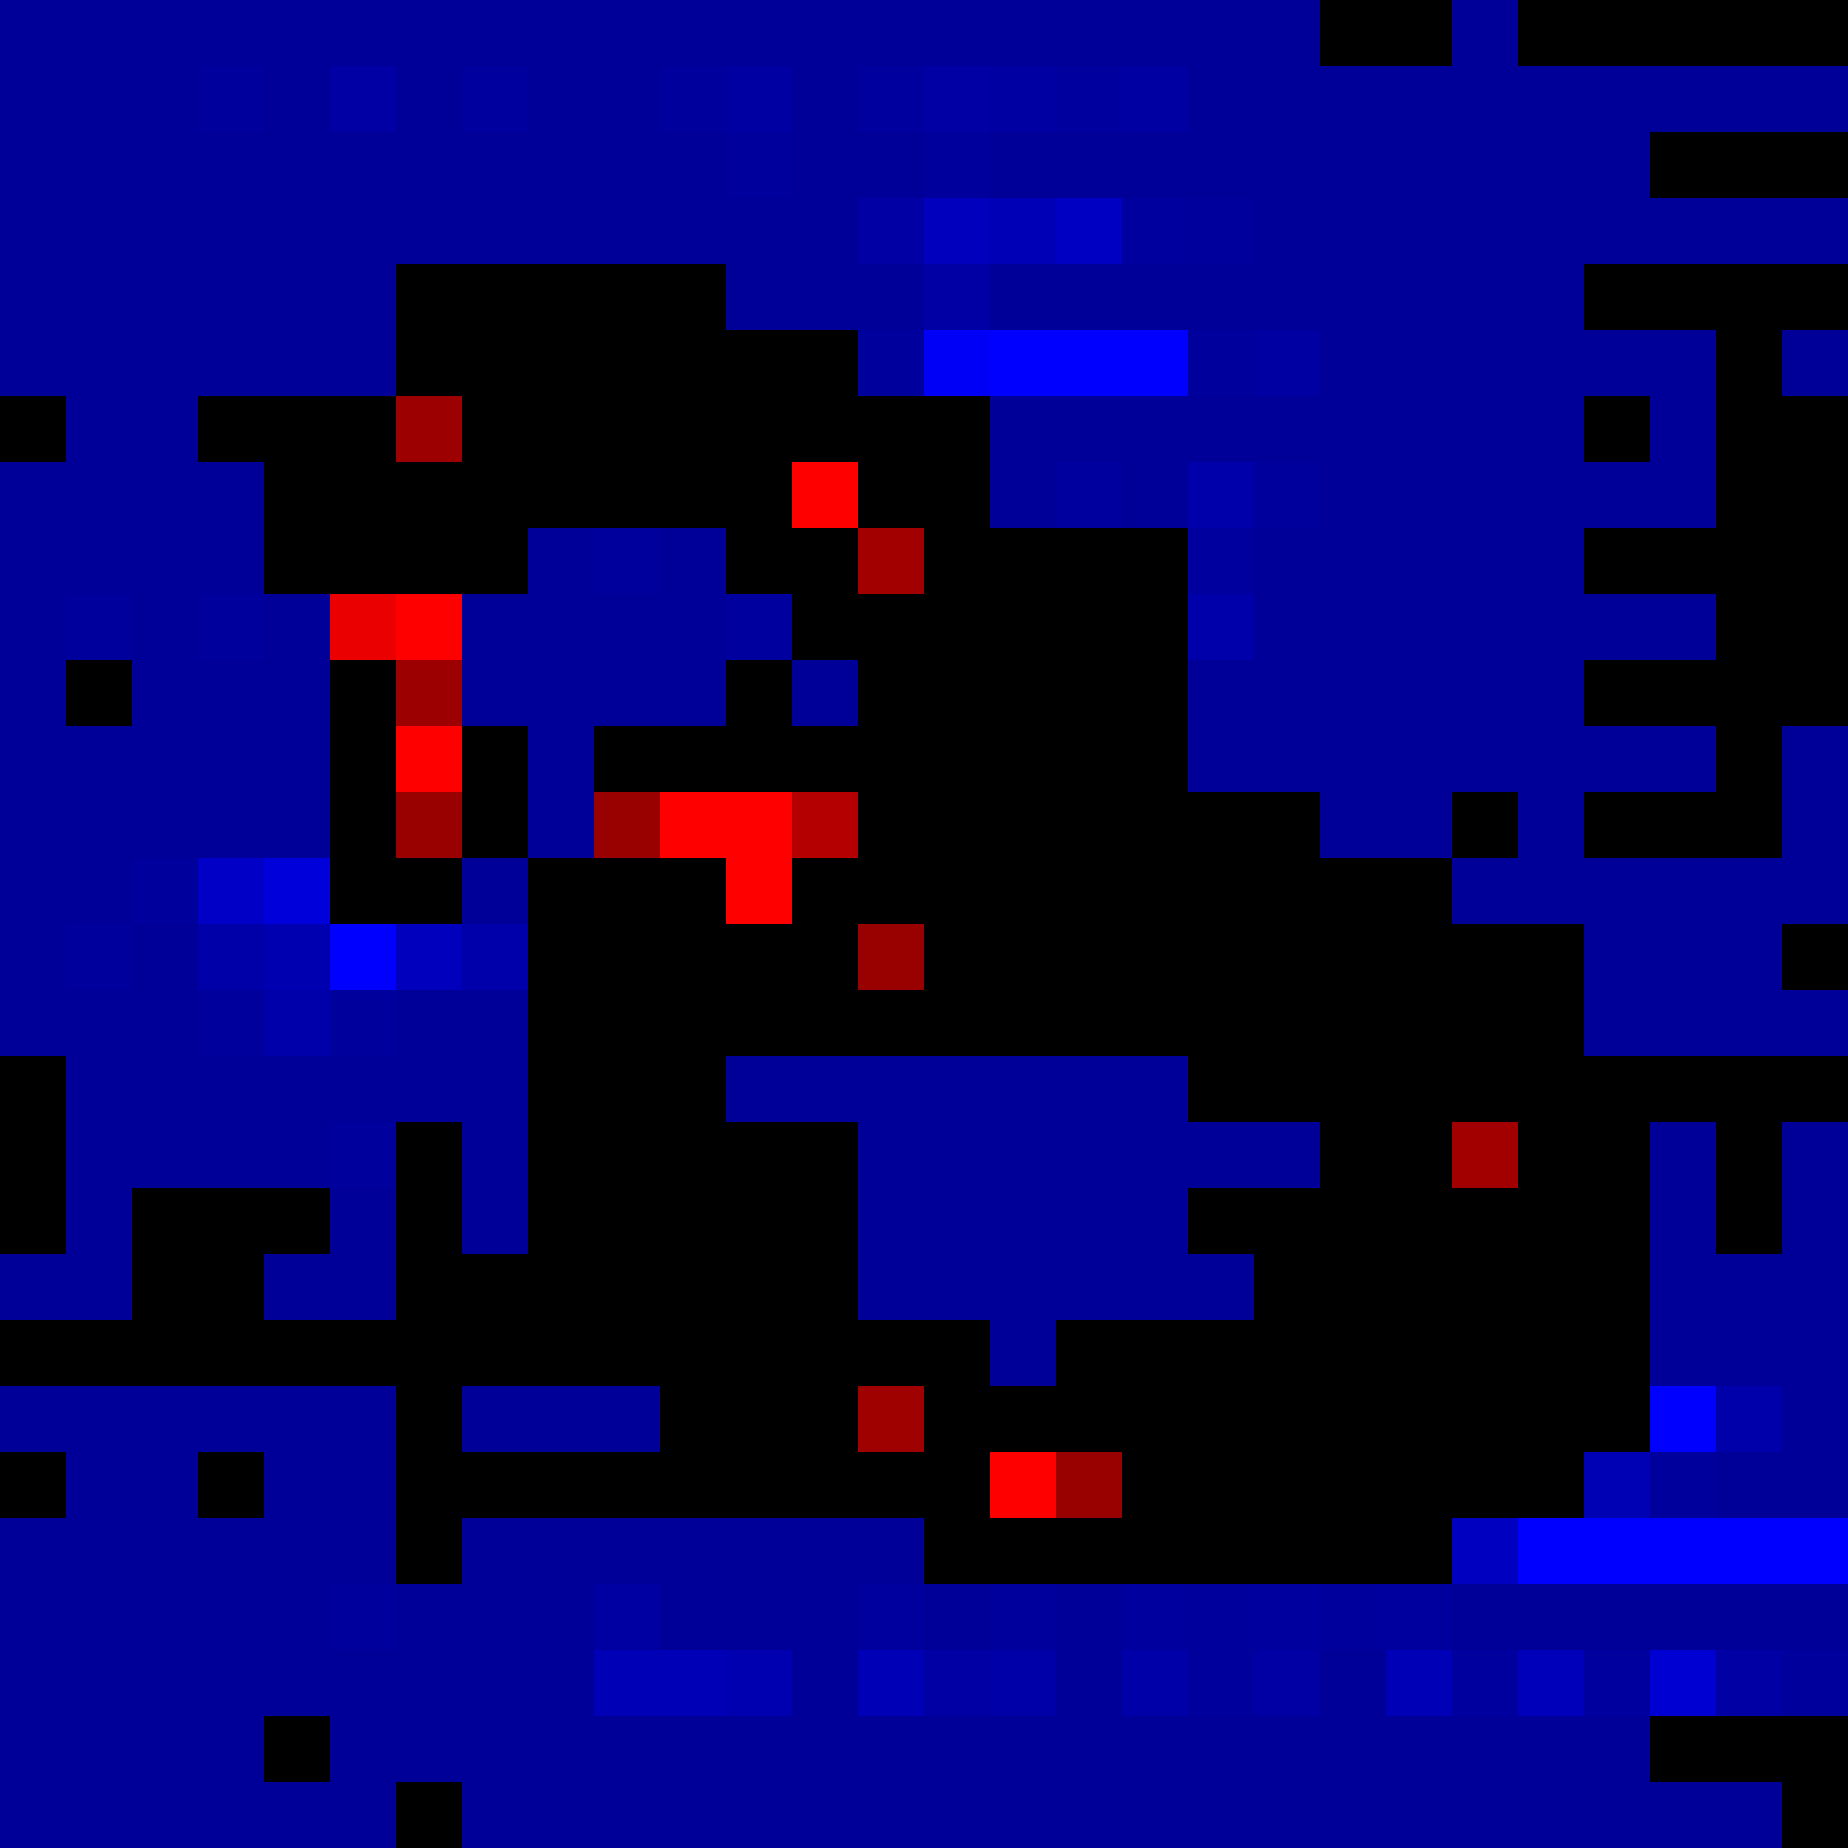
\includegraphics[width=\linewidth]{figures/mnist_split_ic_saliency/image_030_true_3_pred_3/final_saliency_threshold_wrt_5_bright.png}\\[-2pt]{\scriptsize Logit 5}
  \end{minipage}%
  \begin{minipage}[b]{0.19\linewidth}\centering
    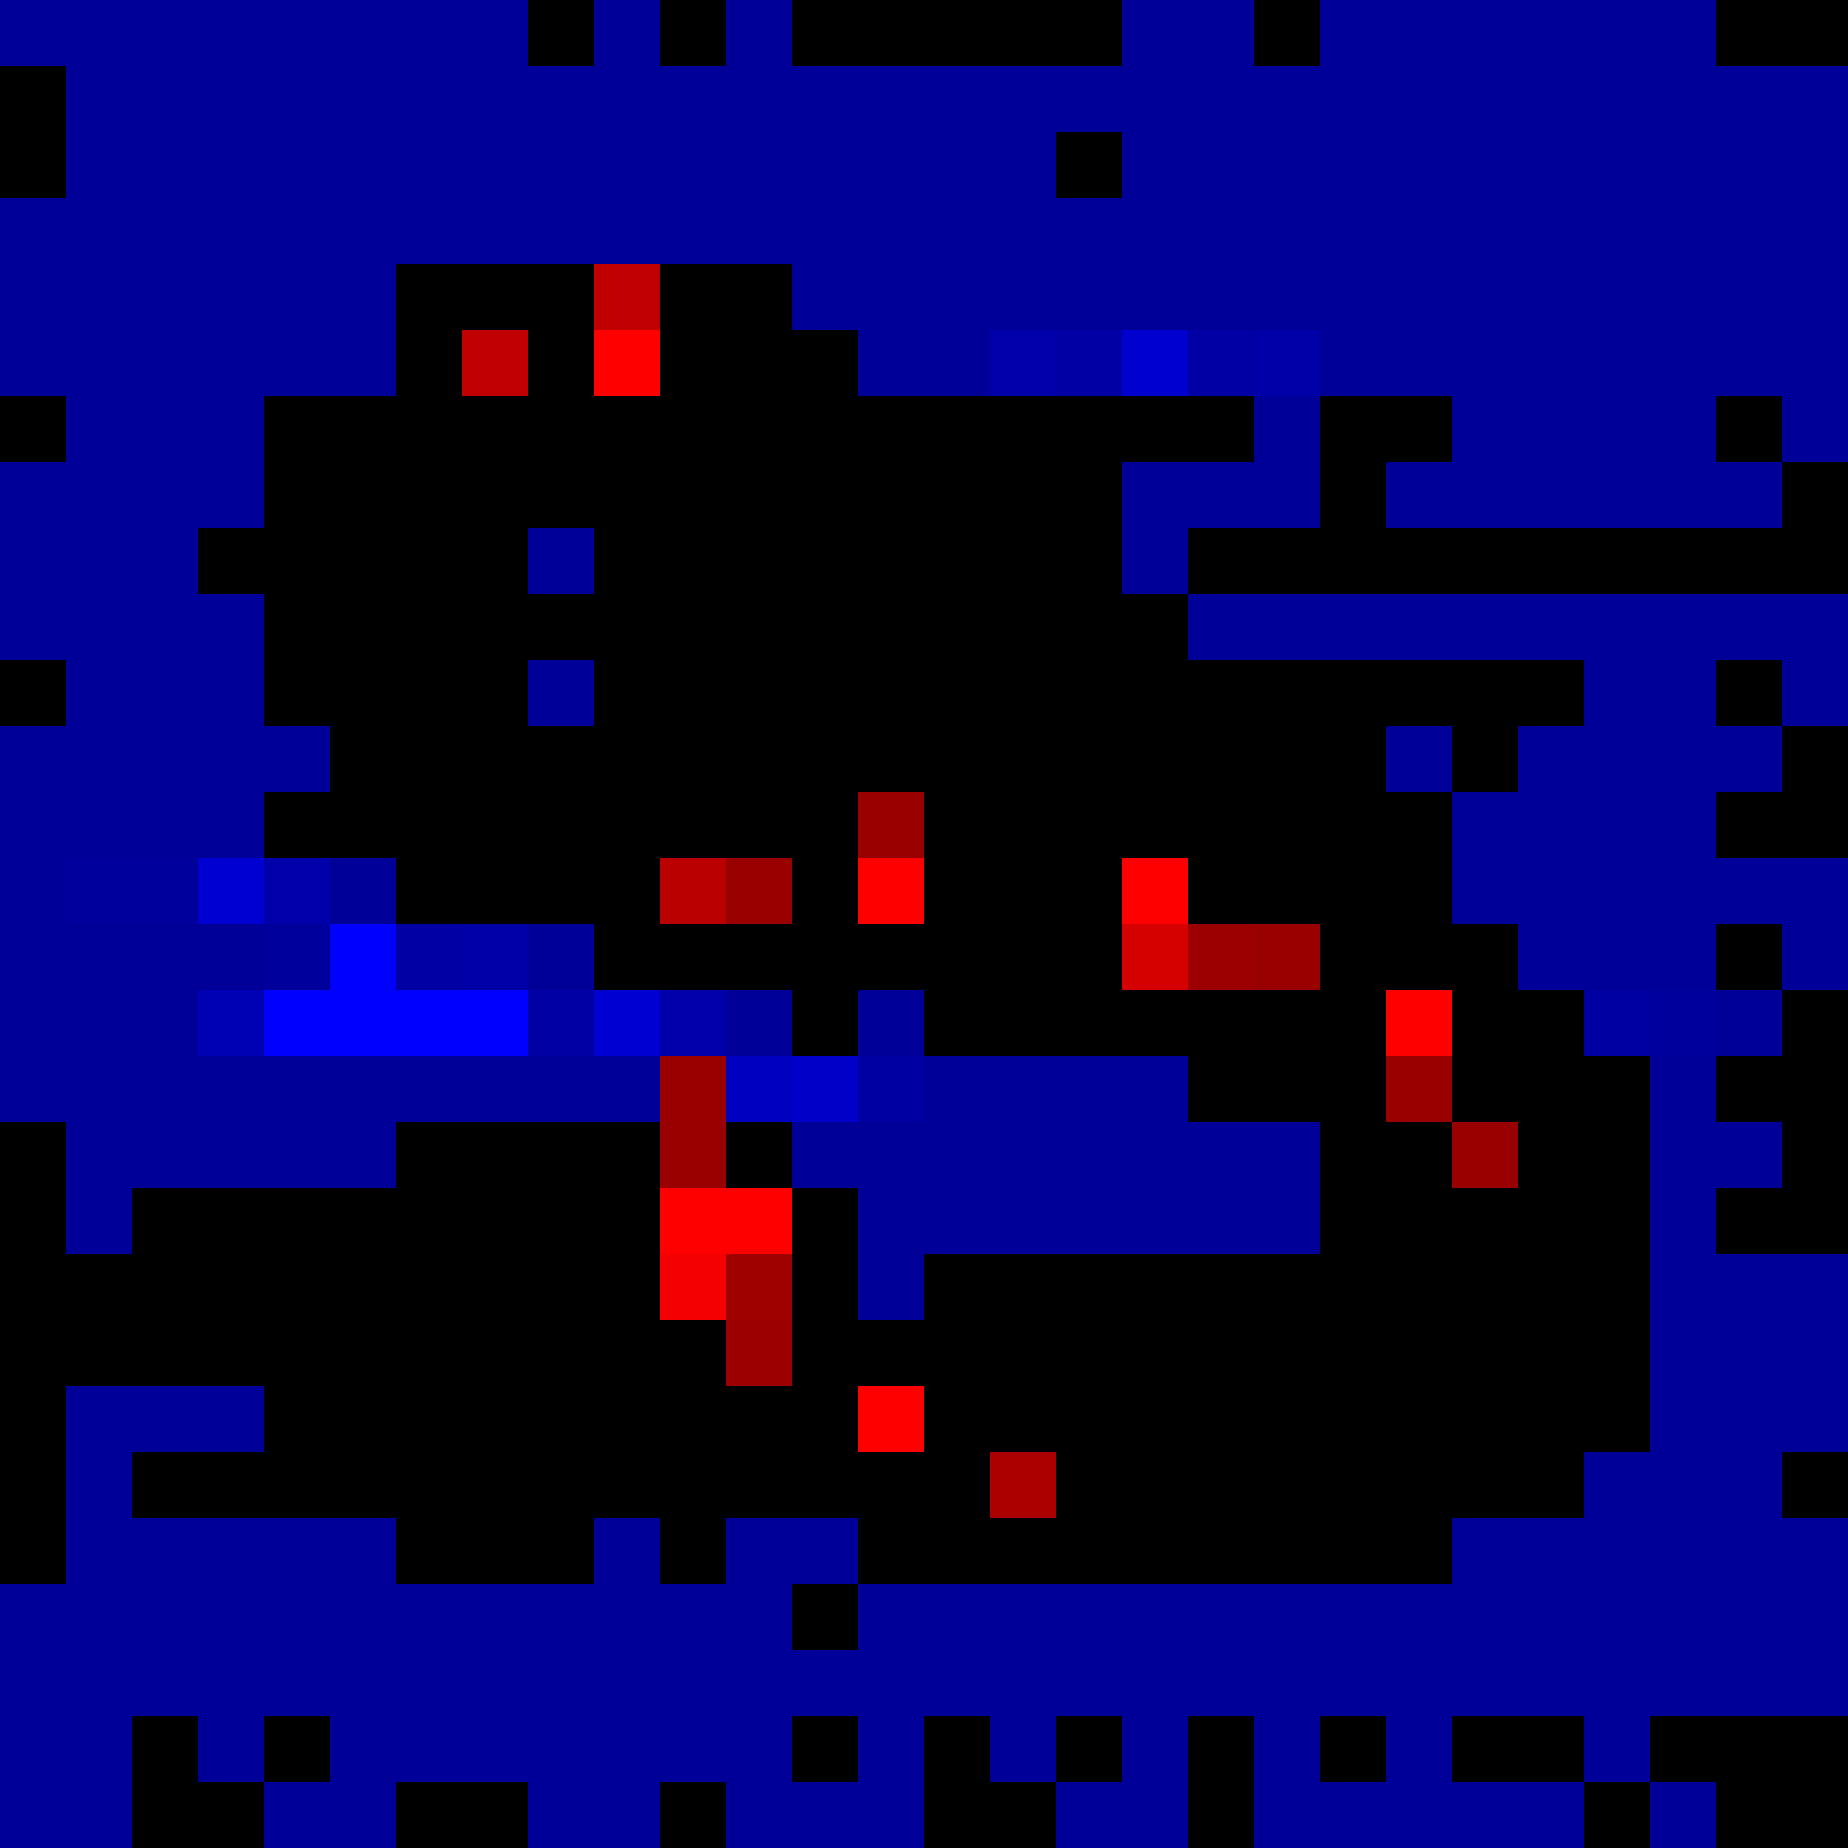
\includegraphics[width=\linewidth]{figures/mnist_split_ic_saliency/image_030_true_3_pred_3/final_saliency_threshold_wrt_6_bright.png}\\[-2pt]{\scriptsize Logit 6}
  \end{minipage}%
  \begin{minipage}[b]{0.19\linewidth}\centering
    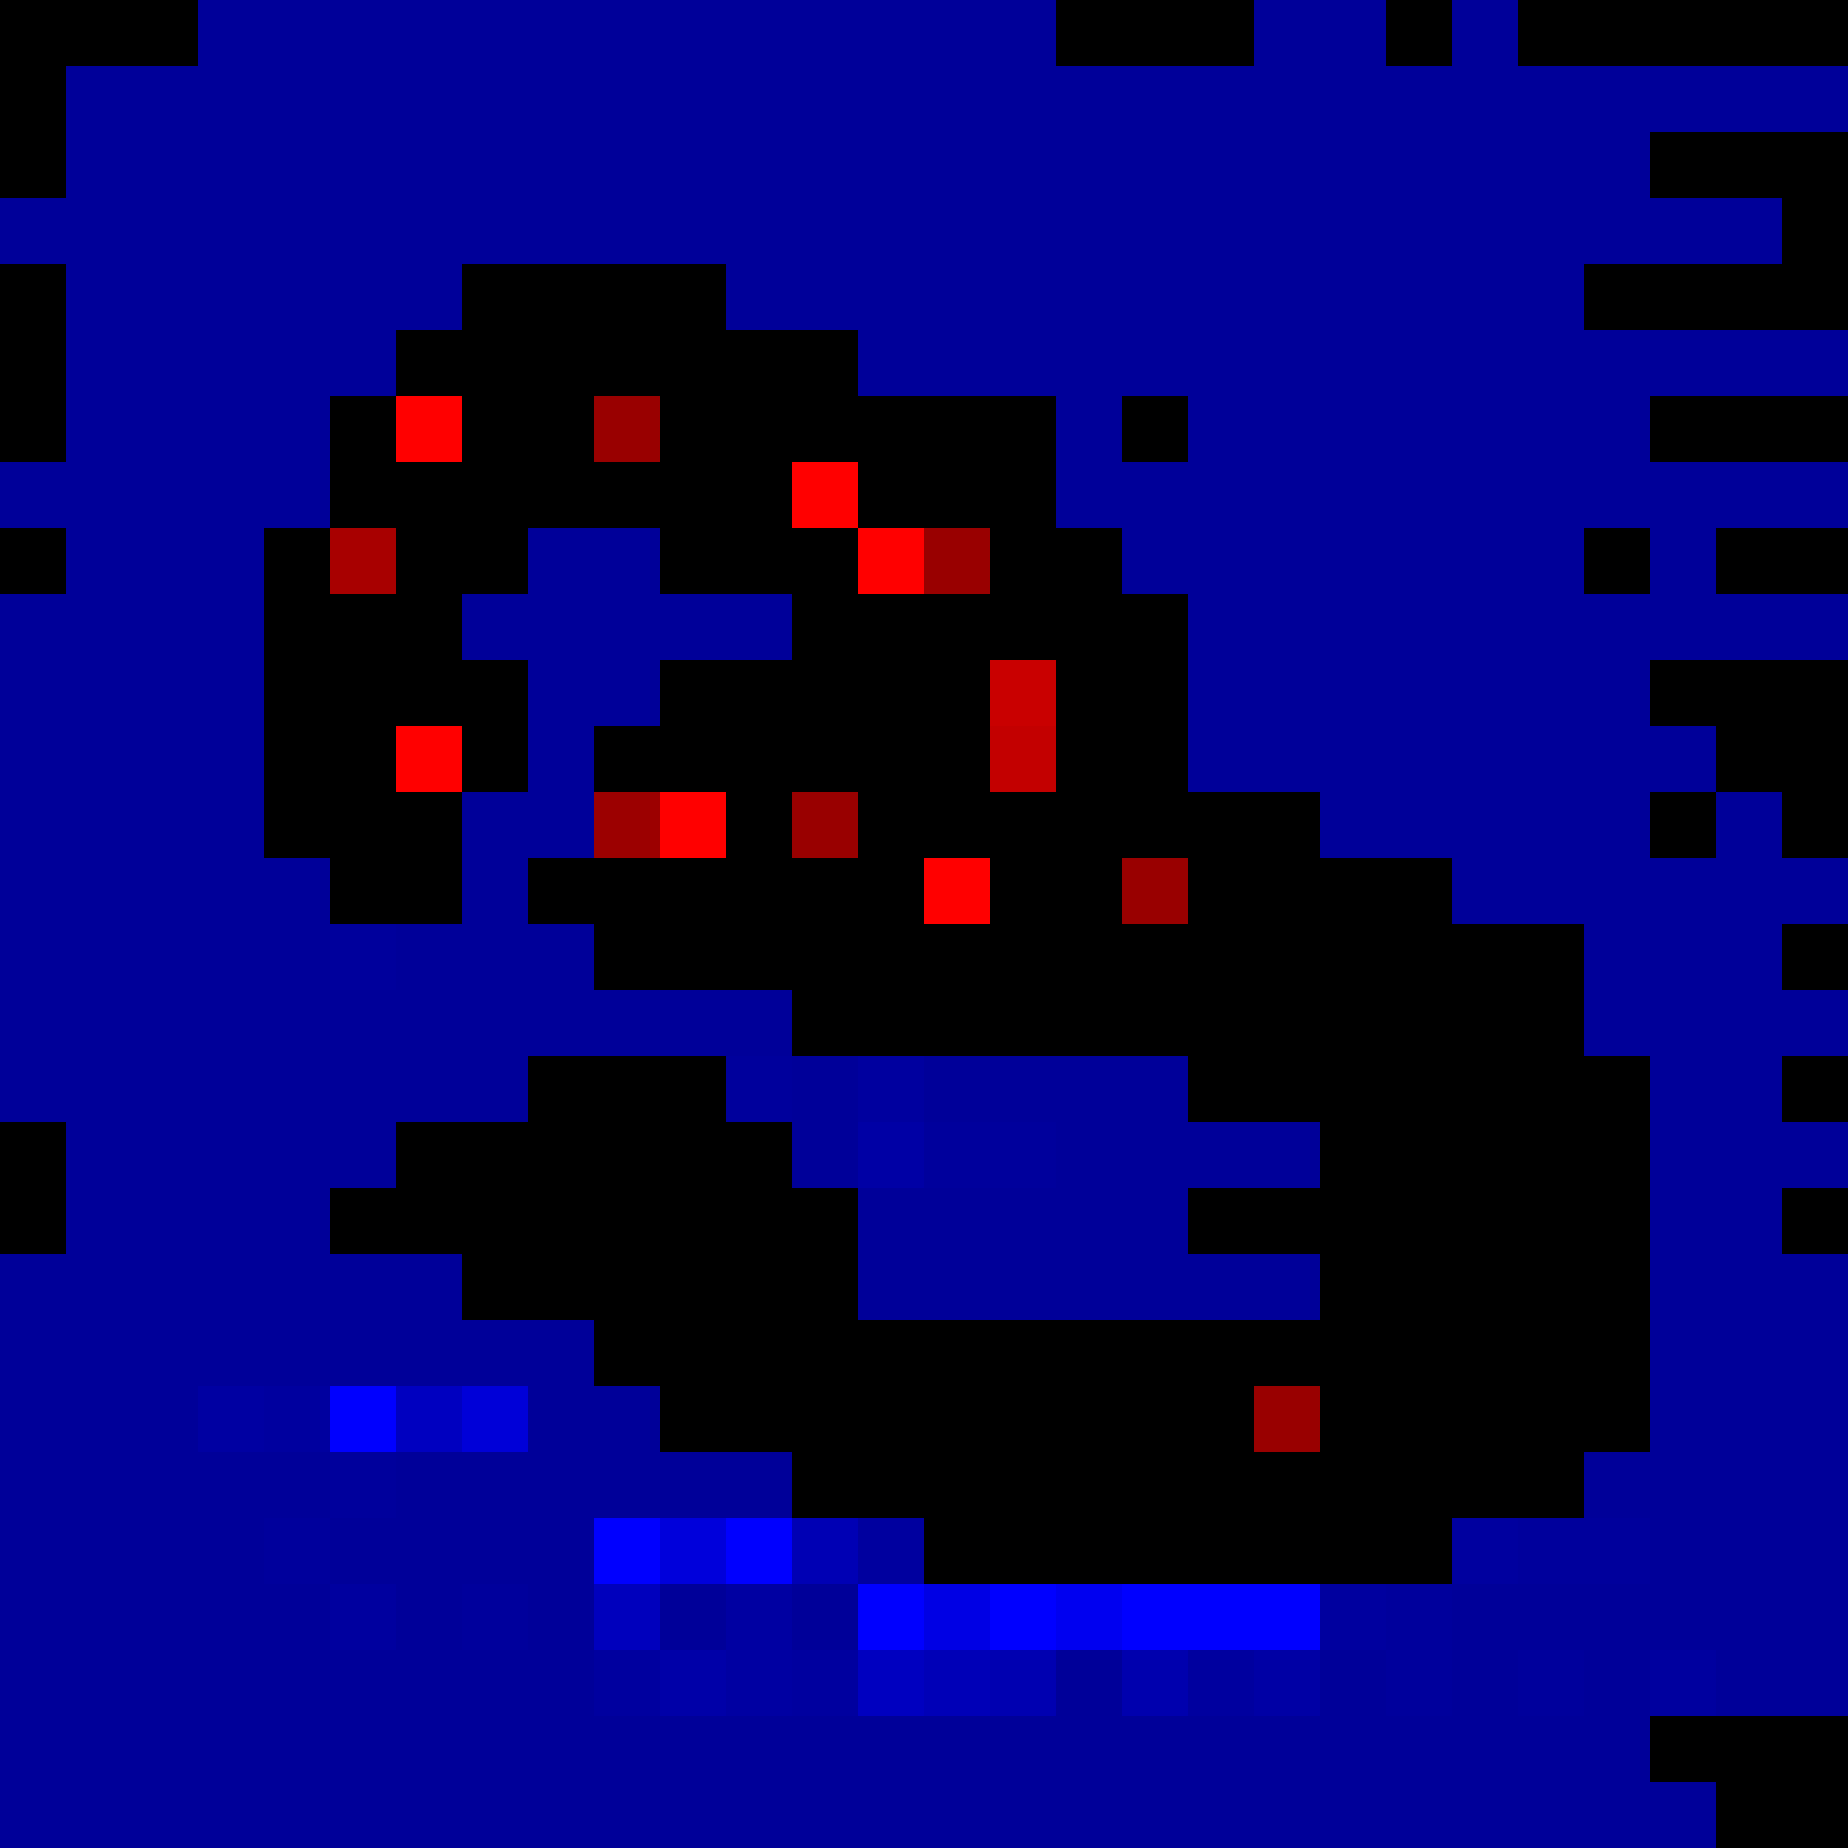
\includegraphics[width=\linewidth]{figures/mnist_split_ic_saliency/image_030_true_3_pred_3/final_saliency_threshold_wrt_7_bright.png}\\[-2pt]{\scriptsize Logit 7}
  \end{minipage}%
  \begin{minipage}[b]{0.19\linewidth}\centering
    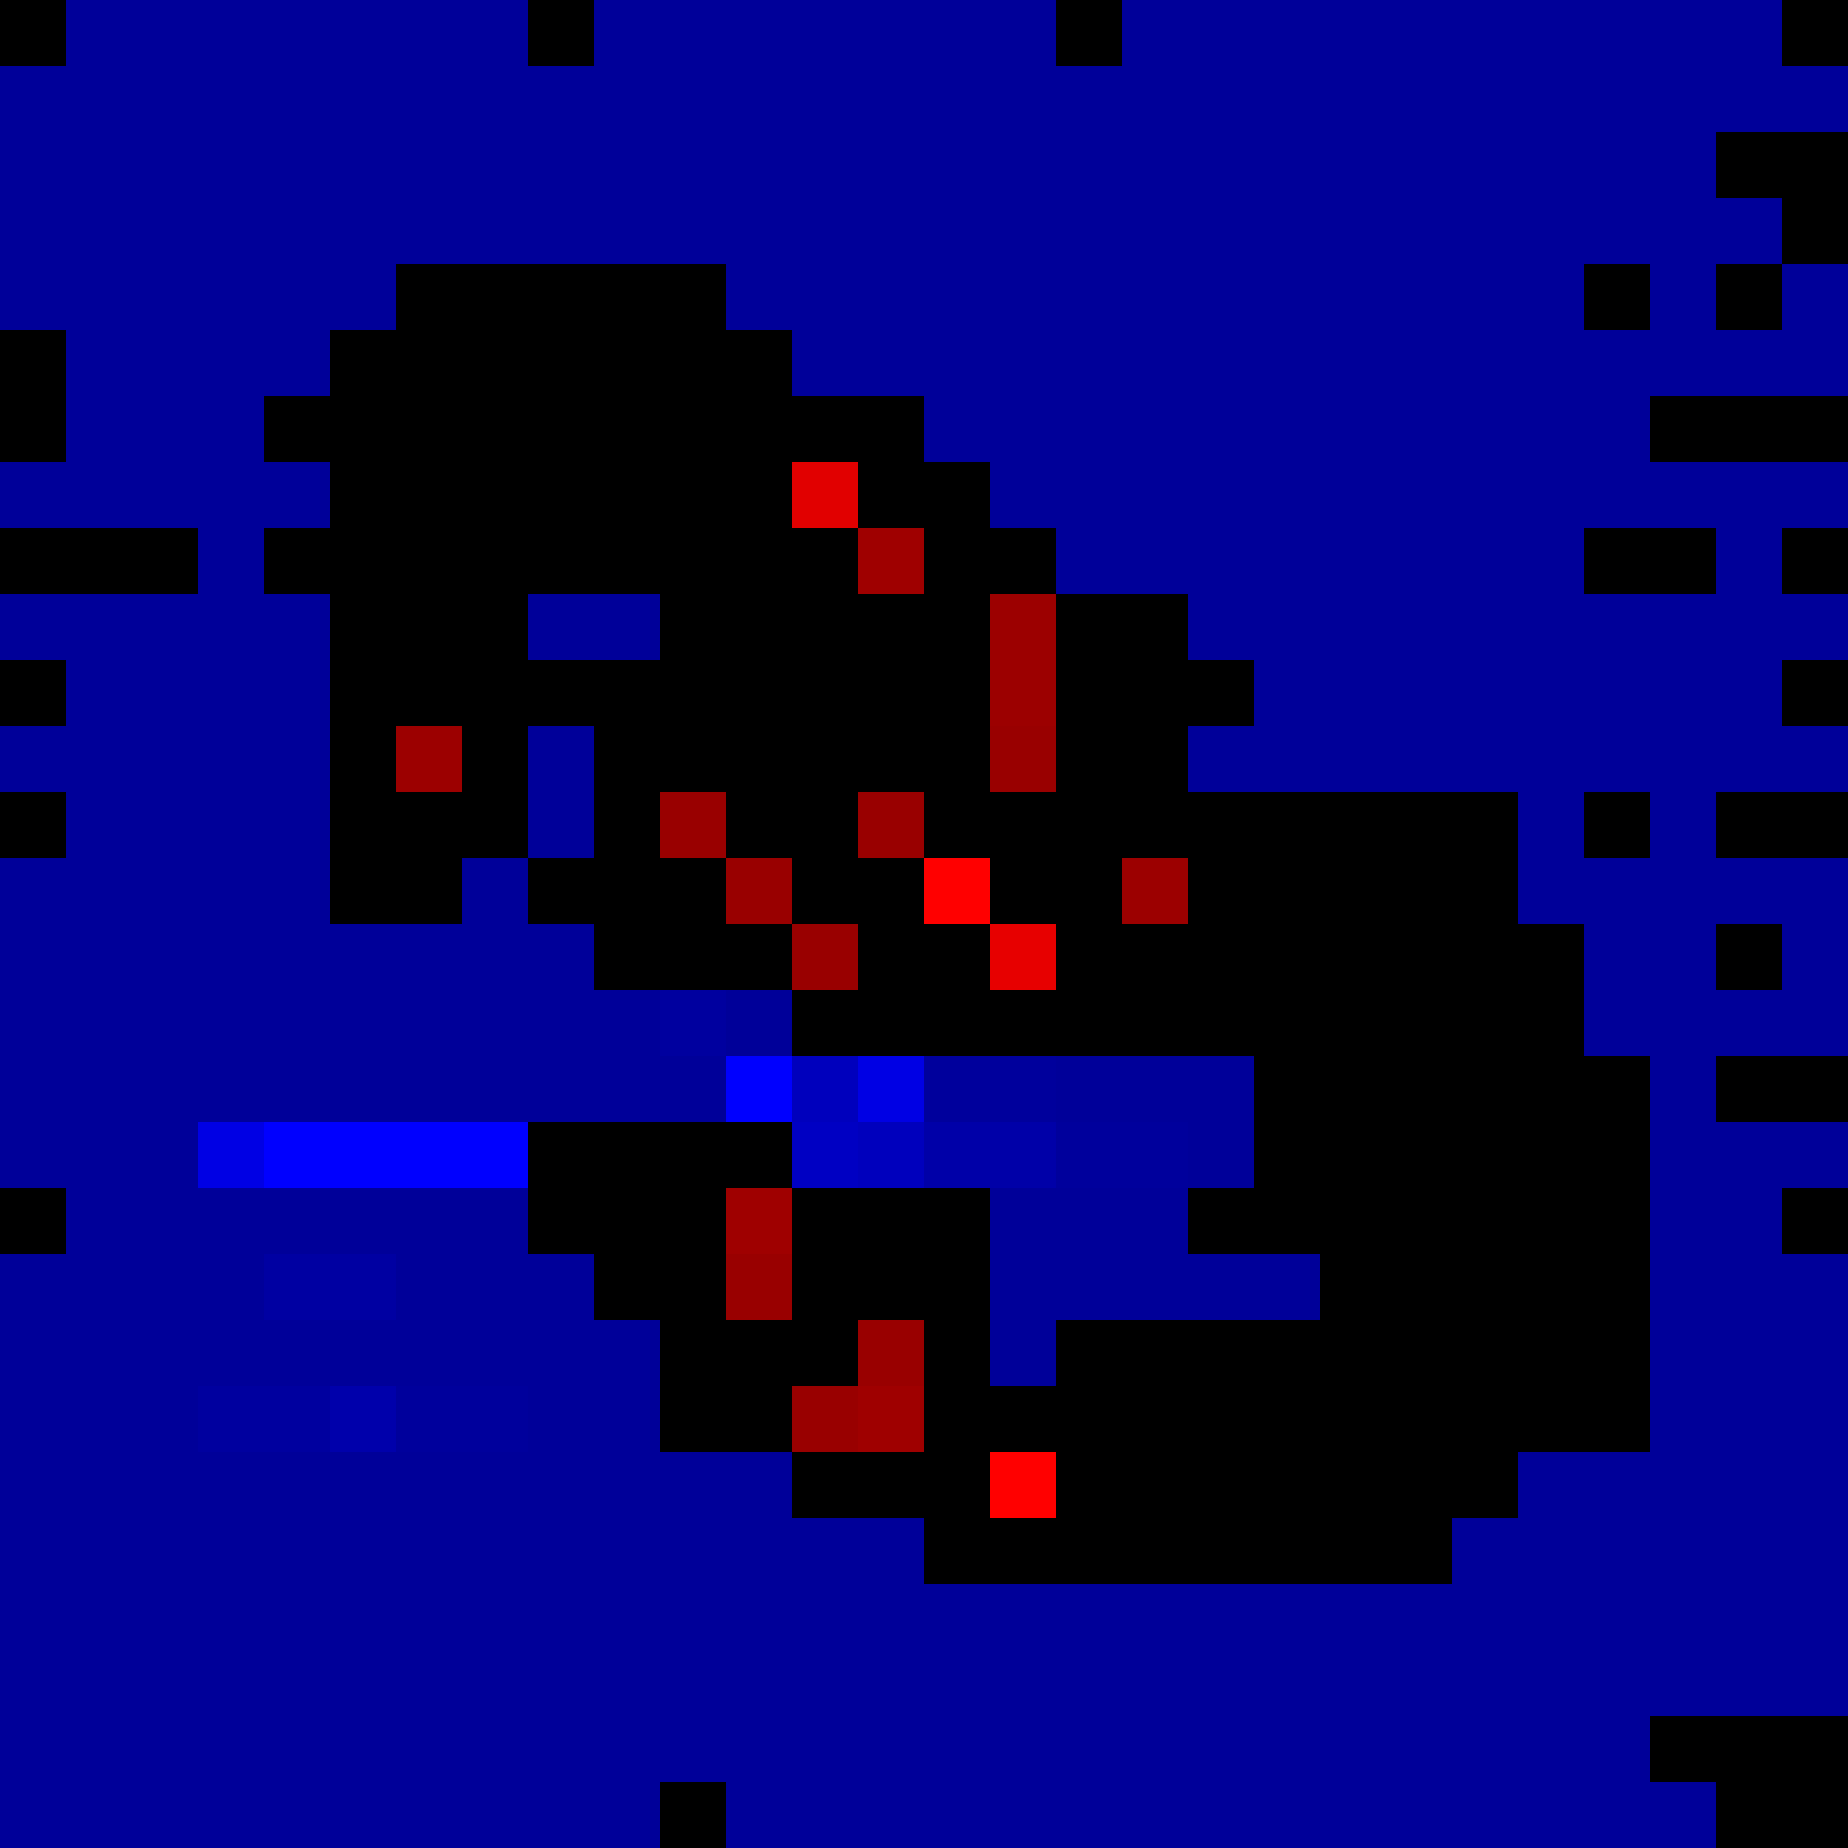
\includegraphics[width=\linewidth]{figures/mnist_split_ic_saliency/image_030_true_3_pred_3/final_saliency_threshold_wrt_8_bright.png}\\[-2pt]{\scriptsize Logit 8}
  \end{minipage}%
  \begin{minipage}[b]{0.19\linewidth}\centering
    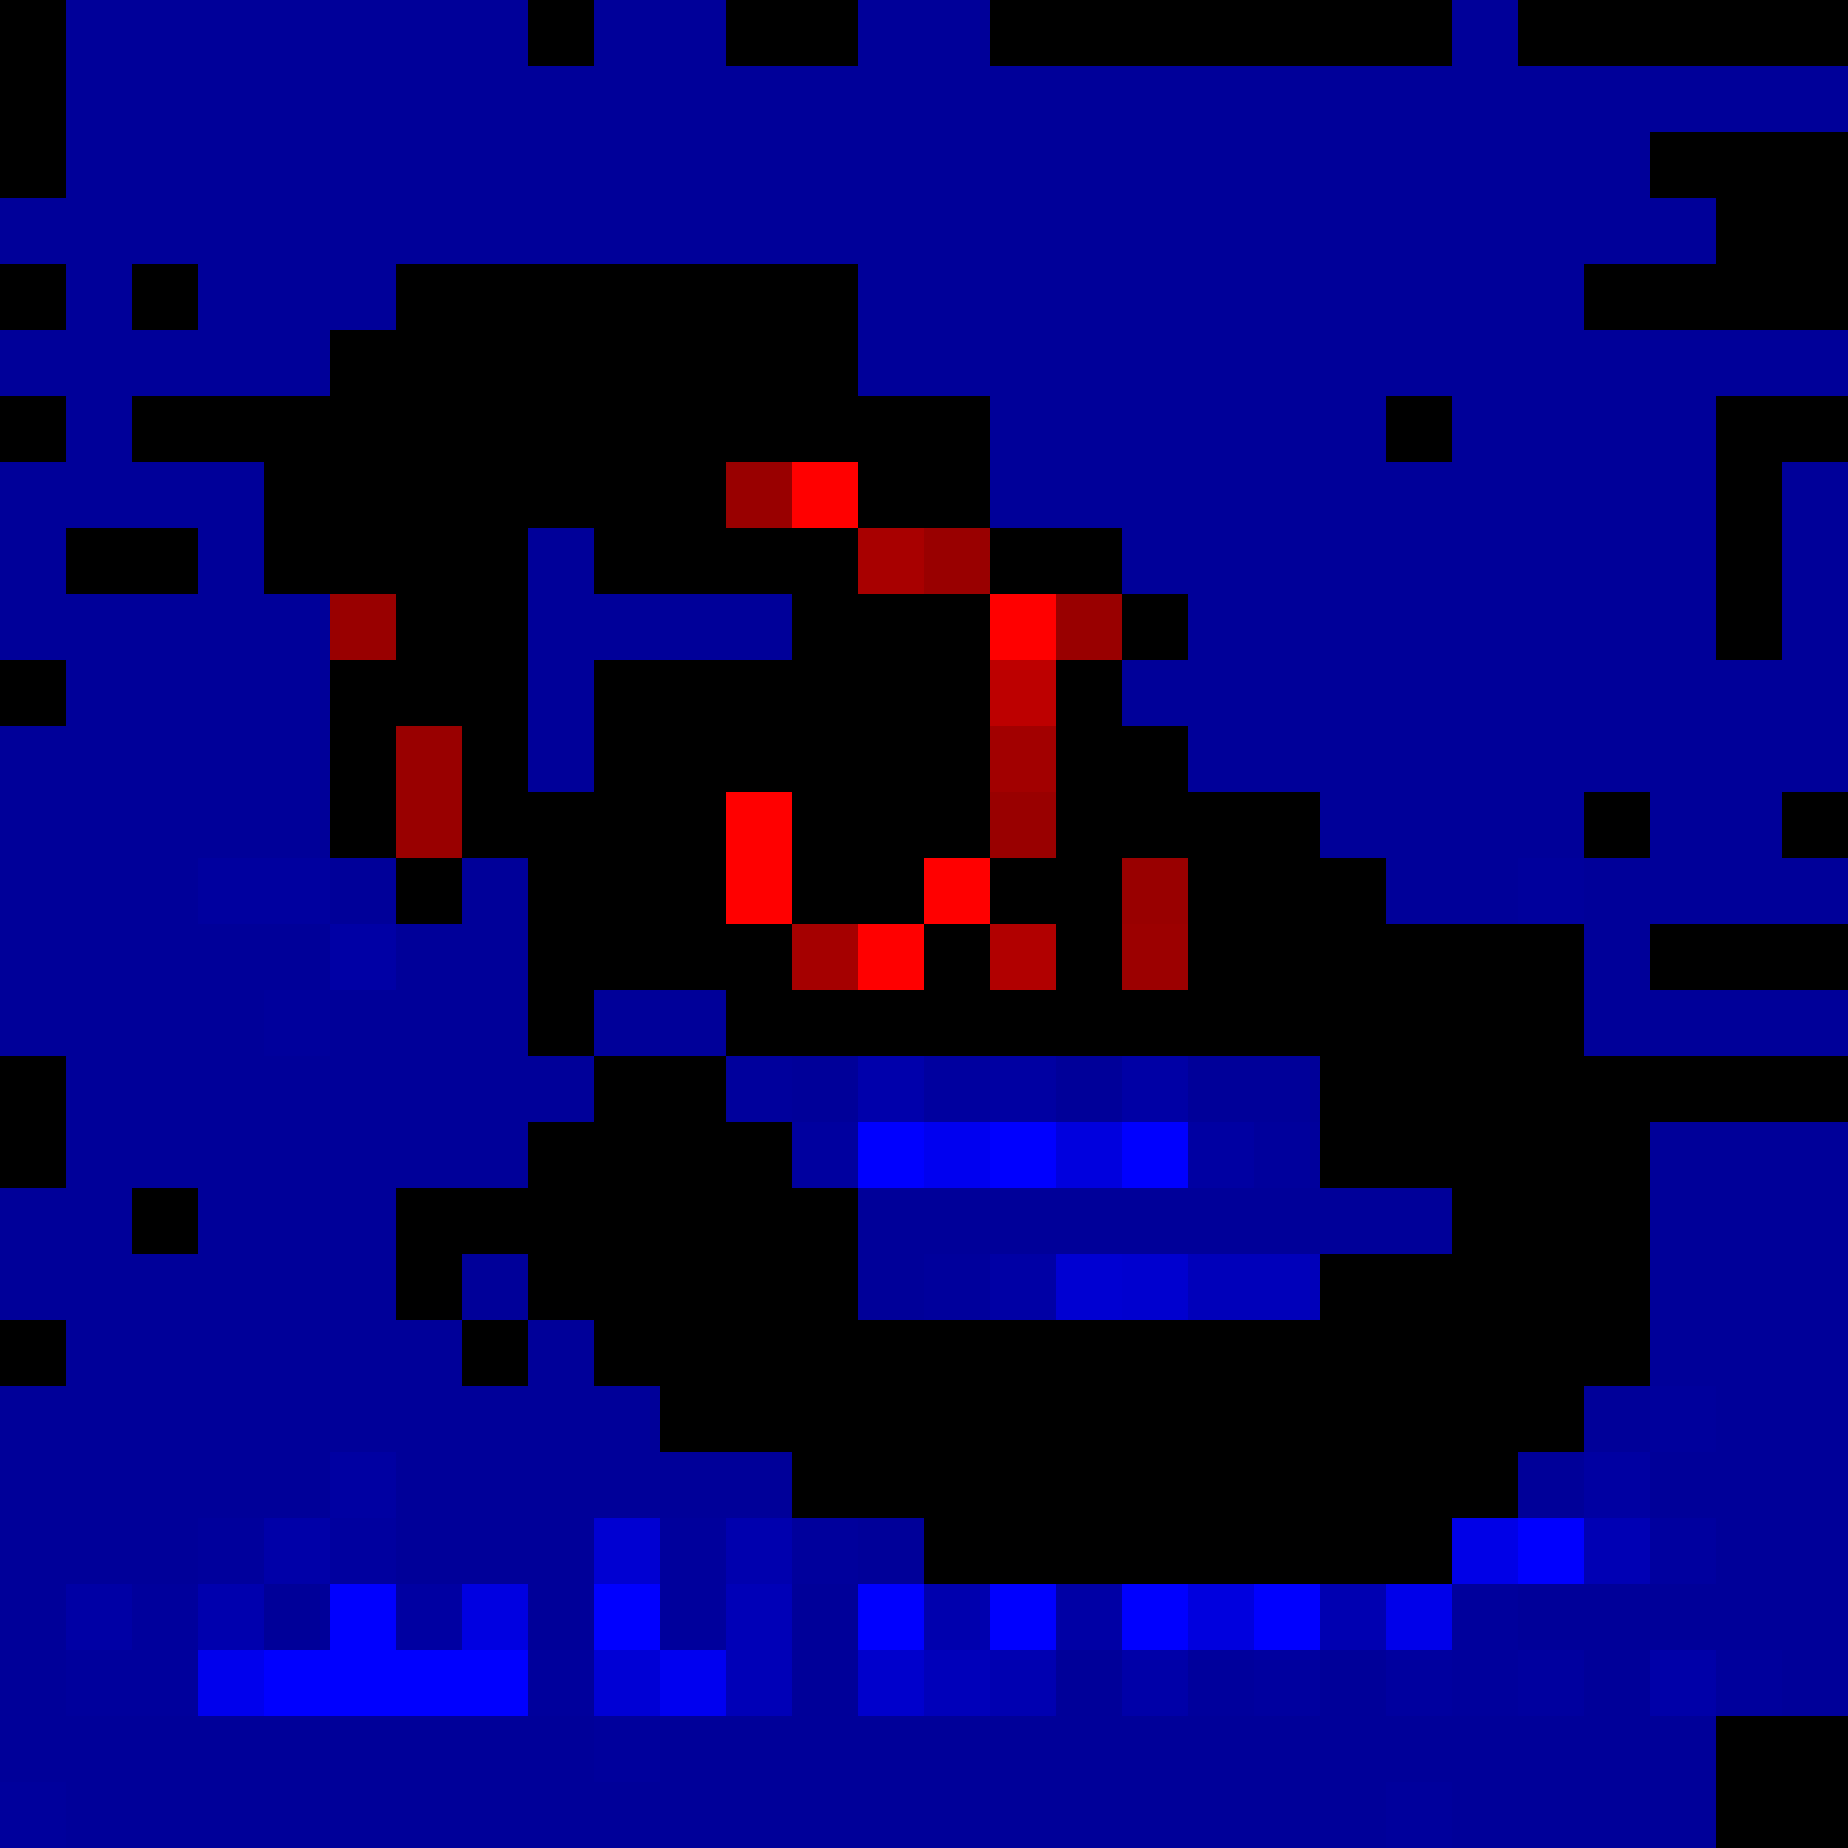
\includegraphics[width=\linewidth]{figures/mnist_split_ic_saliency/image_030_true_3_pred_3/final_saliency_threshold_wrt_9_bright.png}\\[-2pt]{\scriptsize Logit 9}
  \end{minipage}
\end{minipage}

\caption{Combined visualization of the inverted-input DIC stream gradients. The $g$-stream gradient (red) highlights sensitivities on present strokes, while the $h$-stream gradient (blue) highlights sensitivities at candidate missing-stroke locations. These stream-local maps do not by themselves establish the effect of adding pixels on the complete model. On the left: the original digit.}
\label{fig:mnist_split_ic_saliency_main}
\end{figure}
